\chapter{Objetivos}\label{cap.objetivos}
En este capítulo describiremos los objetivos planteados para el Trabajo de Fin de Grado, los requisitos exigidos y la metodología utilizada para el desarrollo.

\section{Problema a abordar}
\label{sec:objetivos}

El objetivo principal de este trabajo es desarrollar una aplicación que a través de técnicas de visión artificial dote de navegación autónoma a un drone real. El resultado consistirá en un despegue, una navegación en tres dimensiones guiada por balizas y por último, una fase de aterrizaje.

Este objetivo global se ha dividido en varios subobjetivos concretos:

\begin{itemize}
	
	\item \textbf{Desarrollo e integración del módulo de autolocalización 3D a partir de balizas visuales:} Este módulo proporciona la posición relativa del drone basándose en la detección de balizas visuales y cálculos geométricos. Dentro del proyecto JdeRobot existe un módulo basado en los trabajos previos mencionados en el capítulo anterior \cite{AlbertoLopez} \cite{ManuelZafra} \cite{JesusSaiz} que será revisado, refinado e integrado en la aplicación final.
	
	\item \textbf{Desarrollo e integración de un módulo de navegación por balizas visuales:} Este módulo será el encargado de buscar y navegar en un entorno real utilizando información del módulo de autolocalización basado en balizas visuales. La navegación deberá ser totalmente autónoma (sin teleoperación).
	
	%\item \textbf{Desarrollo de una aplicación para la calibración de balizas bicolor arlequinadas:} Esta aplicación es fundamental para acelerar el proceso de calibración y de operaciones morfológicas necesarias, a través de una interfaz de usuario sencilla. Generará un fichero de configuración fácilmente transferible que será utilizado por los módulos de despegue y aterrizaje.
	
	%\item \textbf{Implementación e integración de módulos de búsqueda:} Se desarrollarán dos módulos de búsqueda. El primero estará basado en la búsqueda en espiral del TFG de Jorge, siendo necesaria su integración con la aplicación final. El segundo tipo de búsqueda es de tipo rotacional y está utilizará el módulo de autolocalización. El dron girará sobre sí mismo hasta que encuentre la baliza visual que tiene como objetivo.
	
	\item \textbf{Programación del comportamiento del drone  en un autómata de estados finito:} La aplicación final será un único algoritmo basado en un autómata de estados finito que tendrá las siguientes fases: Despegue, aterrizaje, búsqueda y navegación basada en balizas visuales. Esta programación se apoyará en el despegue y aterrizaje existentes en el proyecto de JdeRobot \cite{JorgeVela} \cite{JesusSaiz}, que se refinarán y adaptarán utilizando la herramienta de autómatas \texttt{VisualStates}.
	
	\item \textbf{Validación experimental en el cuadricóptero  real} Se realizarán pruebas unitarias para validar los diferentes módulos constituyentes y pruebas del sistema completo para demostrar el correcto funcionamiento de la solución desarrollada. Se explorarán varias configuraciones ejecutando el software tanto en un ordenador externo como en un ordenador a bordo del cuadricóptero.
	
\end{itemize}

\section{Requisitos}
\label{sec:requisitos}

La solución desarrollada deberá satisfacer, adicionalmente, los siguientes requisitos:

\begin{itemize}
	
	\item Los componentes y aplicaciones desarrollados han de estar integrados en la plataforma JdeRobot-5.6.4.
	
	\item El control de navegación del cuadricóptero ha de ser fluido y ágil, de modo que pueda mantenerse estable al menos 5 segundos en cada baliza, evitando en todo momento perder del campo de visión el objetivo.
	
	\item Los componentes y aplicaciones desarrollados han de ser computacionalmente eficientes y deben ser modulares.
	
	\item El sistema operativo debe estar basado en la distribución GNU/Linux Ubuntu 16.04.
	
	\item Programado en el lenguaje Python, versión 2.7.
	
\end{itemize}

\section{Metodología}

Para materializar los objetivos y requisitos previamente mencionados es necesario aplicar algún método que defina las distintas etapas y estados. En este Trabajo de Fin de Grado se aplica el método de desarrollo en espiral. Este modelo, creado por Barry Boehm en 1986, se utiliza frecuentemente en la ingeniería de software. Se basa en una serie de iteraciones en bucle. En cada ciclo, se realiza un conjunto de cuatro actividades:

\begin{enumerate}
	\item \textbf{Determinar los objetivos}: Poner limitaciones definidas en forma de objetivos o requisitos. Dividir el proyecto en partes más pequeñas.
	\item \textbf{Análisis del riesgo}: Estudiar los riesgos de cada uno de los objetivos que se abordan. Evaluar las alternativas posibles en caso de amenazas.
	\item \textbf{Desarrollar y probar}: Verificación de la tarea actual. Al mismo tiempo, se realiza un análisis para encontrar nuevos factores de riesgo, como errores que se podrían arrastran a la próxima iteración.
	\item \textbf{Planificación}: Establecer y definir las fases anteriores.
\end{enumerate}

\begin{figure}[h]
	\centering
	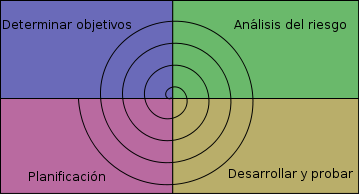
\includegraphics[width=90mm]{imag/desarrollo_en_espiral.png}
	\caption{Representación del desarrollo en espiral.}
	\label{fig:21_planificacion_espiral}
\end{figure}

Durante el desarrollo de este proyecto se han establecido reuniones periódicas con el tutor. En ellas revisábamos los objetivos anteriormente fijados y los resultados obtenidos. Si alguno de los objetivos generaba algún problema o no se llegaba al resultado deseado, se aplazaban o se profundizaba en la raíz del problema. A continuación se determinaban los objetivos de nuestro próximo encuentro. 

Como parte de la evaluación de los objetivos propuestos, ha sido fundamental la utilización del mediawiki\footnote{http://JdeRobot.org/Andresjhe-tfg}  de la plataforma JdeRobot. En él están publicados, a modo de cuaderno de bitácora, los hitos y progresos, incluyendo también imágenes o vídeos. 

Para el seguimiento y almacenamiento del software desarrollado se ha empleado la herramienta de control de versiones GIT. Todo el código relacionado con este proyecto es software libre y es accesible en el repositorio\footnote{https://github.com/RoboticsURJC-students/2014-tfg-Andres-Hernandez}.

\section{Planificación}

Para conseguir los objetivos fijados anteriormente se ha seguido el siguiente plan de trabajo:

\begin{itemize}
	
	\item \textbf{Formación y familiarización con el entorno JdeRobot:} Incluye el preparación de las dependencias necesarias para la instalación del entorno. Estudio de las diferentes bibliotecas, interfaces y componentes. Aprendizaje y profundización de lenguajes de programación como Python y C++, así como la herramienta para las comunicaciones ICE y la biblioteca de visión OpenCV.
	
	\item \textbf{Aprendizaje de la herramienta VisualStates:} Necesaria para la generación de autómatas de estado finito. Se han generado varios ejemplos para conocer las diferentes secciones, para la inserción de variables, funciones y nuevos estados.
	
	\item \textbf{Aprendizaje e implementación del módulo de despegue, búsqueda en espiral y aterrizaje:} Necesario para conocer el funcionamiento del los antecedentes ya existentes de control de un drone para seguir una ruta de control de un drone para aterrizar usando visión. Se ha adaptado y mejorado el código para ganar rendimiento y robusted. También se han buscado soluciones propias de control y se han integrado todos en una máquina de estados finito programada con la herramienta \texttt{VisualStates}.
	
	\item \textbf{Aprendizaje y familiarización con técnicas de autolocalización desde balizas visuales:} Necesario para conocer el funcionamiento de las balizas visuales y cómo obtener las diferentes coordenadas a partir de su detección. Se ha realizado el estudio de antecedentes existentes en el proyecto JdeRobot \cite{AlbertoLopez} \cite{ManuelZafra} junto a la información publicada en la página oficial de AprilTags \footnote{https://april.eecs.umich.edu/}. 
	
	\item \textbf{Validación experimental:} Se ha diseñado una secuencia de pruebas unitarias para poder validar incrementalmente la solución, siendo la última prueba un ejercicio que reunirá y ejecutará de principio a fin las pruebas unitarias anteriormente realizadas y validadas. Ha sido necesaria la instalación de sistema operativo, herramientas y aplicaciones en el co-procesador para poder ejecutar la aplicación final.
	
\end{itemize}
